\documentclass[aspectratio=169]{beamer}

\usepackage[utf8]{inputenc}
\usepackage{lmodern}
\inputencoding{utf8}

\usepackage{tikz}
\usepackage{minted} % syntax highlighting
\usetikzlibrary{positioning}
\usepackage{csquotes}

\definecolor{gris}{rgb}{0.92,0.92,0.92}
\definecolor{blau-upc}{rgb}{.192,.365,.506}

\setbeamercolor{titlelike}{fg=blau-upc}
% \setbeamercolor{barra}{bg=white,fg=white}
\setbeamercolor{capcalera}{bg=blau-upc,fg=white}
\setbeamercolor{section in toc}{fg=blau-upc}
\setbeamertemplate{sections/subsections in toc}[circle]
\setbeamertemplate{itemize items}[circle]
\setbeamercolor{item}{fg=blau-upc}
\setbeamertemplate{blocks}[rounded][shadow=true]
\setbeamercolor*{block body}{bg=gris}
\setbeamerfont{block body}{size=\footnotesize}
\setbeamercolor*{block title}{parent=structure,bg=blau-upc,fg=white}

\setbeamersize{text margin left=12mm,text margin right=12mm}
\setbeamertemplate{navigation symbols}{}

\defbeamertemplate*{headline}{infolines theme}
{
	\begin{beamercolorbox}[wd=\paperwidth,ht=9.5mm,right]{white}%
		
\includegraphics[height=8mm]{./figures/imperial.pdf}\hspace*{1mm}\vskip0.2ex
	\end{beamercolorbox}
% 	\begin{beamercolorbox}[wd=\paperwidth,ht=0.5mm,left]{barra}%
% 		\hspace*{1mm}
% 	\end{beamercolorbox}
}

\setbeamertemplate{footline}
{
	\hbox{
	\begin{beamercolorbox}[wd=0.1\paperwidth,ht=10mm,left]{}
% 		\hspace*{1ex}\includegraphics[height=8mm]{./logotips/imperiallogo.pdf}\vskip 2ex
	\end{beamercolorbox}
	\begin{beamercolorbox}[wd=0.8\paperwidth,ht=3ex,center]{}
		\hspace*{4ex}\insertsection\vskip 4ex
	\end{beamercolorbox}
	\begin{beamercolorbox}[wd=0.1\paperwidth,ht=3ex,right]{}
		\insertpagenumber\hspace*{6ex}\vskip 4ex
	\end{beamercolorbox}
	}
}

\setbeamertemplate{title page}
{
	\vbox{}
	\vfill
	\begin{centering}
		{\usebeamerfont{title}\usebeamercolor[fg]{title}\inserttitle}
		\vskip0.2em
		{\usebeamerfont{subtitle}\usebeamercolor[fg]{subtitle}\insertsubtitle}
		\vskip2em\par
		\small\insertauthor\par
		\vskip0.7em\par
		\tiny\insertdate\vskip1em\par
	\end{centering}
% 	\vfill
}


%%%%%%%%%%%%%%%%%%%%%%%%%%%%%%%%%%%%%%%%%
% University Assignment Title Page 
% LaTeX Template
% Version 1.0 (27/12/12)
%
% This template has been downloaded from:
% http://www.LaTeXTemplates.com
%
% Original author:
% WikiBooks (http://en.wikibooks.org/wiki/LaTeX/Title_Creation)
%
% License:
% CC BY-NC-SA 3.0 (http://creativecommons.org/licenses/by-nc-sa/3.0/)
% 
%
%%%%%%%%%%%%%%%%%%%%%%%%%%%%%%%%%%%%%%%%%
%----------------------------------------------------------------------------------------
%	PACKAGES AND OTHER DOCUMENT CONFIGURATIONS
%----------------------------------------------------------------------------------------
%\usepackage[a4paper,hmargin=2.8cm,vmargin=2.0cm,includeheadfoot]{geometry}
%\usepackage{textpos}
%\usepackage[backend=bibtex,sorting=none]{biblatex}
%\usepackage{tabularx,longtable,multirow,subfigure,caption}%hangcaption
%\usepackage{fncylab} %formatting of labels
%\usepackage{fancyhdr} % page layout
%\usepackage{url} % URLs
%\usepackage[english]{babel}
%\usepackage{amsmath}
%\usepackage{graphicx}
%\usepackage{dsfont}
%\usepackage{epstopdf} % automatically replace .eps with .pdf in graphics
%\usepackage{array}
%\usepackage{latexsym}
%\usepackage[pdftex,hypertexnames=false,colorlinks]{hyperref} % provide links in pdf

% additional

\usepackage{caption}

%%%%%% TITLE, AUTHOR, DATE DEFINITIONS %%%%%%
\title{Making Smart Contracts Safer}
\author{
    Aurel Bílý, 
    Catalin Craciun,
    Calin Farcas,\\
    Constantin Mueller, 
    Yicheng Luo, 
    Niklas Vangerow
}
\date{\today}
%%%%%%

% A macro to create a slide and section at the same time
\newcommand{\sectionslide}[1]{%
  \section{#1}
  \begin{frame}
  \begin{center}
    \vbox{}
    {\LARGE \usebeamercolor[fg]{title} #1}
    \par
  \end{center}
  \end{frame}
}

\begin{document}

\begin{frame}
\titlepage
\end{frame}

\sectionslide{Introduction}
% FIRST SIXTY SECONDS
% Smart contracts have the potential to be a hugely disruptive technology. 
% They are decentralised applications that could transform areas such as banking, 
% insurance and even our voting system. 
% At the moment, most smart contracts are written in Solidity, 
% a language with many flaws considering smart contracts need to be very safe,
% as once deployed they can never be changed.
% Because of this, Franklin Schrans developed Flint under Susan's supervision. 
% Flint is a programming language for smart contracts aimed to be much safer while being simple to use. 
% However, Flint was not usable in practice due to the lack of essential features. 
% For our third-year group project we worked on adding those features and 
% improving the Flint ecosystem to make Flint more useful in the real world.*

{ % all template changes are local to this group.
    \setbeamertemplate{navigation symbols}{}
    \begin{frame}[plain]
        \begin{tikzpicture}[remember picture,overlay]
            \node[at=(current page.center)] {
                
\includegraphics[width=\paperwidth]{figures/generic_image.jpg}
            };
        \end{tikzpicture}
     \end{frame}
}

\sectionslide{Problems with Smart Contracts}

% To give you an idea of Flint is and what smart contracts are, here is 
% a very simple example of one that works as a lottery.
% The creator initialises the smart contract with a ticket price and a winning
% number threshold used to determine a winner.
% Anyone can then send currency to the contract which sends back the entire jackpot
% if the owner wins. Everyone can verify the smart contract for themselves and knows
% that it cannot change, so the system does not rely on trust unlike lotteries 
% where you need to trust the organisers not to tamper with the numbers.
% We can think about a smart contract
% as a REST web interface as shown by the diagram on the right.
\begin{frame}
\frametitle{Example Contract - Lottery}
\begin{columns}
\begin{column}{0.5\textwidth}
  \inputminted[fontsize=\tiny]{swift}{code/lottery.flint}
\end{column}
\begin{column}{0.5\textwidth}
  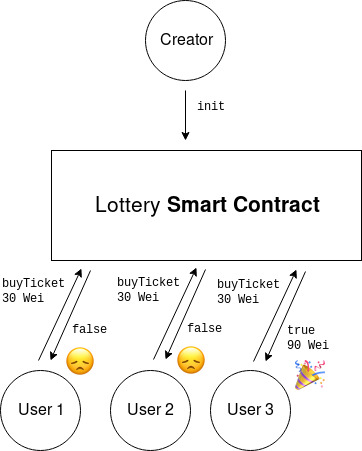
\includegraphics[scale=0.4]{figures/lottery_diagram.jpg}
\end{column}
\end{columns}
\end{frame}


% Codes snippets like the one with saw just now run on the Ethereum Virtual Machine, or
% EVM for short. As you can imagine, writing EVM byte-code is not fun, a bit like 
% writing assembly code by hand. You might know about the Solidity programming 
% language, which aimed to simplify writing smart contracts; it's something like the 
% PHP or JavaScript of smart contract programming languages, as it has few safety features.
% Flint is an attempt to create a less error-prone programming
% language. The underpinning philosophy is simplicity, and its design has been 
% largely inspired by Swift. Creating a safe language involves 
% prohibiting many avoidable programmer errors at compile-time. At the
% moment, these avoidable errors put hundreds of millions of dollars
% worth of cryptocurrencies at risk.
\begin{frame}{Problems with Ethereum Smart Contracts}
    \begin{itemize}
        \item Smart contracts are \textbf{immutable}
        \item Smart contracts are difficult to program with existing technologies
        \item Smart contracts \textbf{really need to be safe} as they directly handle currency
        \item Solidity does not provide a good solution as it lacks safety checks and features
        \item[$\Rightarrow$] Flint aims to be safer
    \end{itemize}
\end{frame}

\sectionslide{Issues with Flint}
% As mentioned before, as of October, there were still serious flaws with Flint.
% In particular, Flint did not allow for external calls, i.e. function calls to
% other contracts, which are an absolute necessity to process currency.
% In plain words, Flint cannot be used to develop smart contracts without external calls.
% In addition, Flint - like Solidity - used to treat Ether as integers which 
% could easily lead to "losing" currency. Remember that a contract is entirely controlled
% by its code and that the code is immutable.
% Also, Flint had no real ecosystem for development and 
% no unit testing, meaning that there
% were plenty of additions and improvements for us to make.
\begin{frame}{Issues with Flint}
    \begin{itemize}
        \item No interaction with other smart contracts due to lack of external calls
        \item Programmers may `lose' currency as it is modelled as simple integers
        \item Flint lacked a development ecosystem and unit testing
        \item[$\Rightarrow$] Our goal was to improve all these aspects of Flint
    \end{itemize}
\end{frame}

\sectionslide{Achievements}
% We will now go through our achievements in this project.

\subsection{Asset Traits with Self}

\begin{frame}{What are Asset Traits?}
\centering\mintinline{swift}{struct trait Asset { ... }}
\\

\begin{itemize}
    \item Flint traits are similar to Java's interfaces
    \item Captures the commonalities between different assets, like {\tt Wei}
\end{itemize}
% Reducing duplication prevents a programmer from forgetting
%   to implement safety precautions necessary for functions such as `transfer`
\end{frame}

\begin{frame}{What are Asset Traits?}
\centering
\inputminted{swift}{code/asset-transfer-function.flint}
\end{frame}


\begin{frame}{Cross-Asset Transfers}
% One thing that we want to prevent is one asset being transferred to another
% This can be done with a polymorphic self type or generics. 
% We chose not to implement generics due to our time on the project being limited o
% and them being complex, going against the language principle of simplicity.

\begin{columns}
\begin{column}{0.5\textwidth}
  \begin{block}{Not allowed}
    \inputminted{swift}{code/ca-not-allowed.flint}
  \end{block}
\end{column}
\begin{column}{0.5\textwidth}
  \begin{block}{Allowed}
    \inputminted{swift}{code/ca-allowed.flint}
  \end{block}
\end{column}
\end{columns}

\end{frame}

\begin{frame}{Polymorphic Self}
% Rather than implementing generics in the language, we implemented a 
% polymorphic self type.
% As you can see, Self is treated as the implementing type at the calling site,
% but functions in place of the trait in the context of the trait.
% example of type signatures
\inputminted{swift}{code/polymorphic-self.flint}
\end{frame}

\subsection{General Improvements}
% We have also implemented/fixed/improved a number of smaller features, many of which were found while trying to solve different problems.
\begin{frame}
\frametitle{General Improvements}
\begin{itemize}
    \item Right associativity of the dot operator
    \item Unification of event and function declaration syntax
    \item Function calls parameter passing/ordering
    \item Testing
\end{itemize}
\end{frame}

\begin{frame}
% Unified the declaration syntax for events and functions to increase clarity.
\frametitle{Events and Functions}
\begin{itemize}
    \item Unify the declaration syntax
    \item Implement default parameters for functions
\end{itemize}
    \begin{columns}
        \begin{column}{0.5\textwidth}
            \begin{block}{Before}
	        \inputminted[fontsize=\small]{swift}{code/events-before.flint}
	        \end{block}
        \end{column}
        \begin{column}{0.5\textwidth}
            \begin{block}{After}
	        \inputminted[fontsize=\small]{swift}{code/events-after.flint}
	        \end{block}
        \end{column}
    \end{columns}
\end{frame}

\begin{frame}
% We came up with new logic for checking function call argument types, including for default parameters. We are also now enforcing labels and Swift-like ordering for parameters.
\frametitle{Function Call Parameters}
\begin{itemize}
    \item Improved logic for parameter checking (includes default parameters)
    \item Enforce labels and Swift-like ordering
\end{itemize}
\end{frame}

\subsection{Unit Testing}
\begin{frame}{Why Test?}
\begin{itemize}
    \item Not all features implemented
    \item Tests only cover parts of the codebase, and test end-to-end
    \item No way to tell whether features have regressed
    \item Less manual testing, more confidence
\end{itemize}
% After working on the compiler for a few weeks, it became increasingly clear
% that many of the features that we had assumed were implemented, were only
% implemented partially.
% Due to a lack of unit tests, we had no way to know whether our features
% worked in isolation, whether there were any regressions
% We also had to verify that our new additions worked by testing manually
% There was a test suite but it only tested the whole compiler, making problems hard to debug
\end{frame}

\begin{frame}{The Road to Mocking}
\begin{center}
    \begin{itemize}
        \item Mocking and stubbing like JMock
        \item Swift has read-only reflection
        \item Cuckoo was outdated and did not work on Linux
    \end{itemize}
\end{center}
% we wanted to support mocking and stubbing like JMock.
% swift only has read-only reflection, requiring all stubs to be declared 
%   at compile-time rather than dynamically at runtime like JMock.
% We wanted to use code generation to create these stubs before compilation.
% We tried several approaches, including implementing this code generation ourselves
%   before finding Cuckoo, a framework that implements an API similar to JMock.
% Cuckoo is a framework that we wanted to integrate, but it was outdated
%   as the swift ecosystem is immature and packages are not regularly updated.
% We had to update Cuckoo and many of its dependencies to work on Swift 4.2 and 
%   to retain compatibility with Linux
% Cuckoo employs powerful code generation
\end{frame}

\begin{frame}{Testing Framework}
\begin{columns}
    \begin{column}{0.4\textwidth}
        \inputminted[fontsize=\tiny]{swift}{code/unit-test.flint}
    \end{column}
    \begin{column}{0.6\textwidth}
        \begin{itemize}
            \item XCTest integrated into Xcode and SPM
            \item Code requires extensive refactoring to make testing possible
            \item TDD approach used
        \end{itemize}
    \end{column}
\end{columns}
% For our overall testing framework, we chose XCTest as it was integrated into Xcode and the Swift package manager.
% We did not end up writing a lot of tests because we wanted to implement more features. 
% The code is also written in a manner that requires refactoring into distinct units to make testing them in isolation possible.
% For some features we took a Test Driven Development approach, developing a test and seeing it fail before covering the case in the implementation.
\end{frame}

% These feed into the Demo
\subsection{Language Server Protocol}

% LSP is a clean way to implement IDE integration, by having just one implementation of a protocol that all IDEs support. The way it works is pretty simple, the IDE is sending some events and the LSP server returns back actions or content.
\begin{frame}
\frametitle{Language Server Protocol}
\begin{figure}
    \centering
    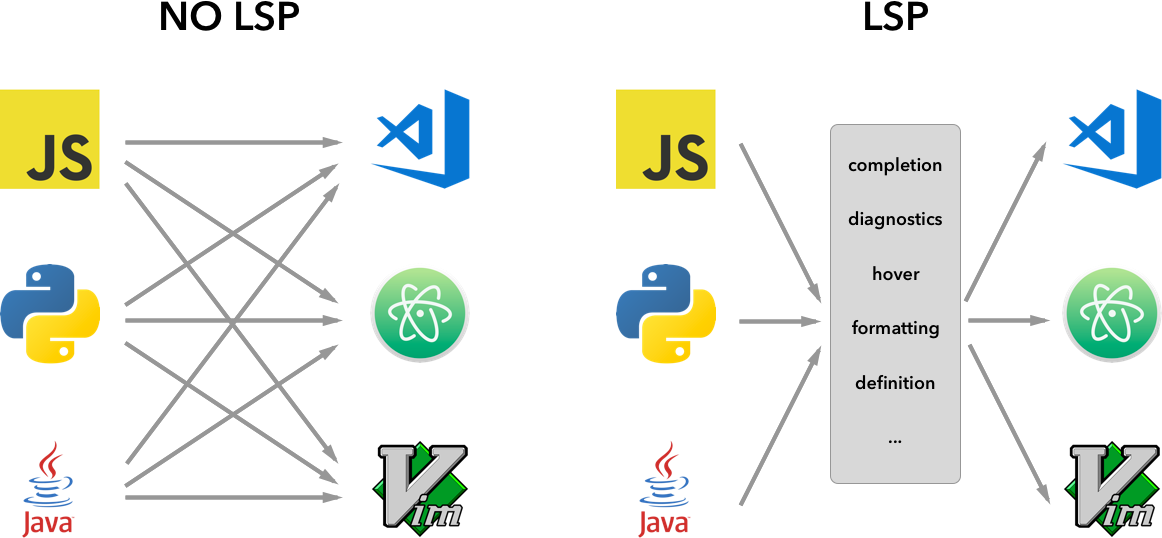
\includegraphics[width=0.6\textwidth]{figures/lsp.png}
    \caption* {LSP architecture \\ \tiny {https://code.visualstudio.com/api/language-extensions/language-server-extension-guide}}
\end{figure}
\end{frame}

% One of the main highlights here is the wiring of the LS with the flint compiler. We initially implemented it as compilation when the user manually saves the file, but what we really wanted was to have auto-compilation. This was probably the trickiest part, since LSP does not support it by default, so we had to simulate it. Since every LSP message is processed asynchronously, we were able to sleep inside the thread for our 2 second period of time and then check if any messages came through while the thread was sleeping. If no messages came through, we would save the "file string" to a temporary location and run the flint compiler on it.
\begin{frame}
\frametitle{LSP - Compilation and Auto-saving}
\begin{itemize}
    \item Wire LSP to use the flintc compiler for bringing compilation errors and warnings into the editor
    \item Initially compiling when the user saves the file
    \item Implement auto-compilation when the user stops editing the file for 2 seconds
    \begin{itemize}
        \item LSP not supporting it by default
        \item should not interfere with auto-saving
        \item 'temporary file' implementation and thread sleeping
    \end{itemize}
\end{itemize}
\end{frame}

\begin{frame}
\begin{figure}
\frametitle{LSP - Auto-Compilation}
    \centering
    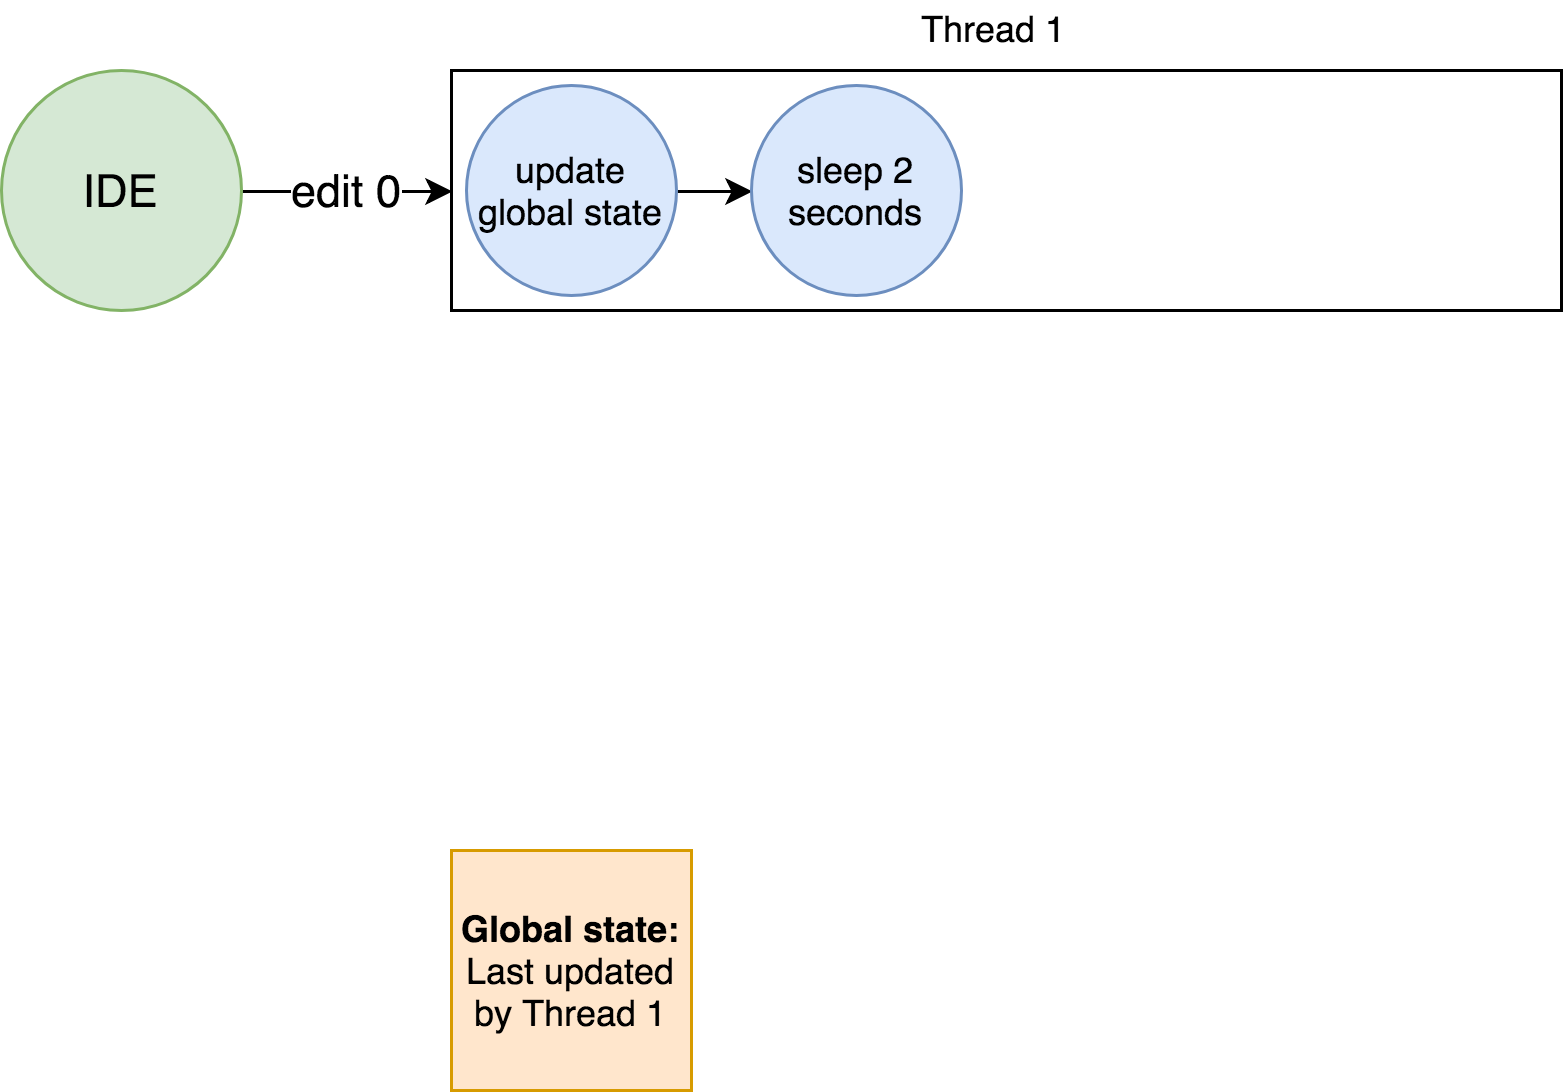
\includegraphics[width=0.6\textwidth]{figures/lsp-step-1.png}
    \caption*{Auto-Compilation Step 1}
\end{figure}
\end{frame}

\begin{frame}
\begin{figure}
\frametitle{LSP - Auto-Compilation}
    \centering
    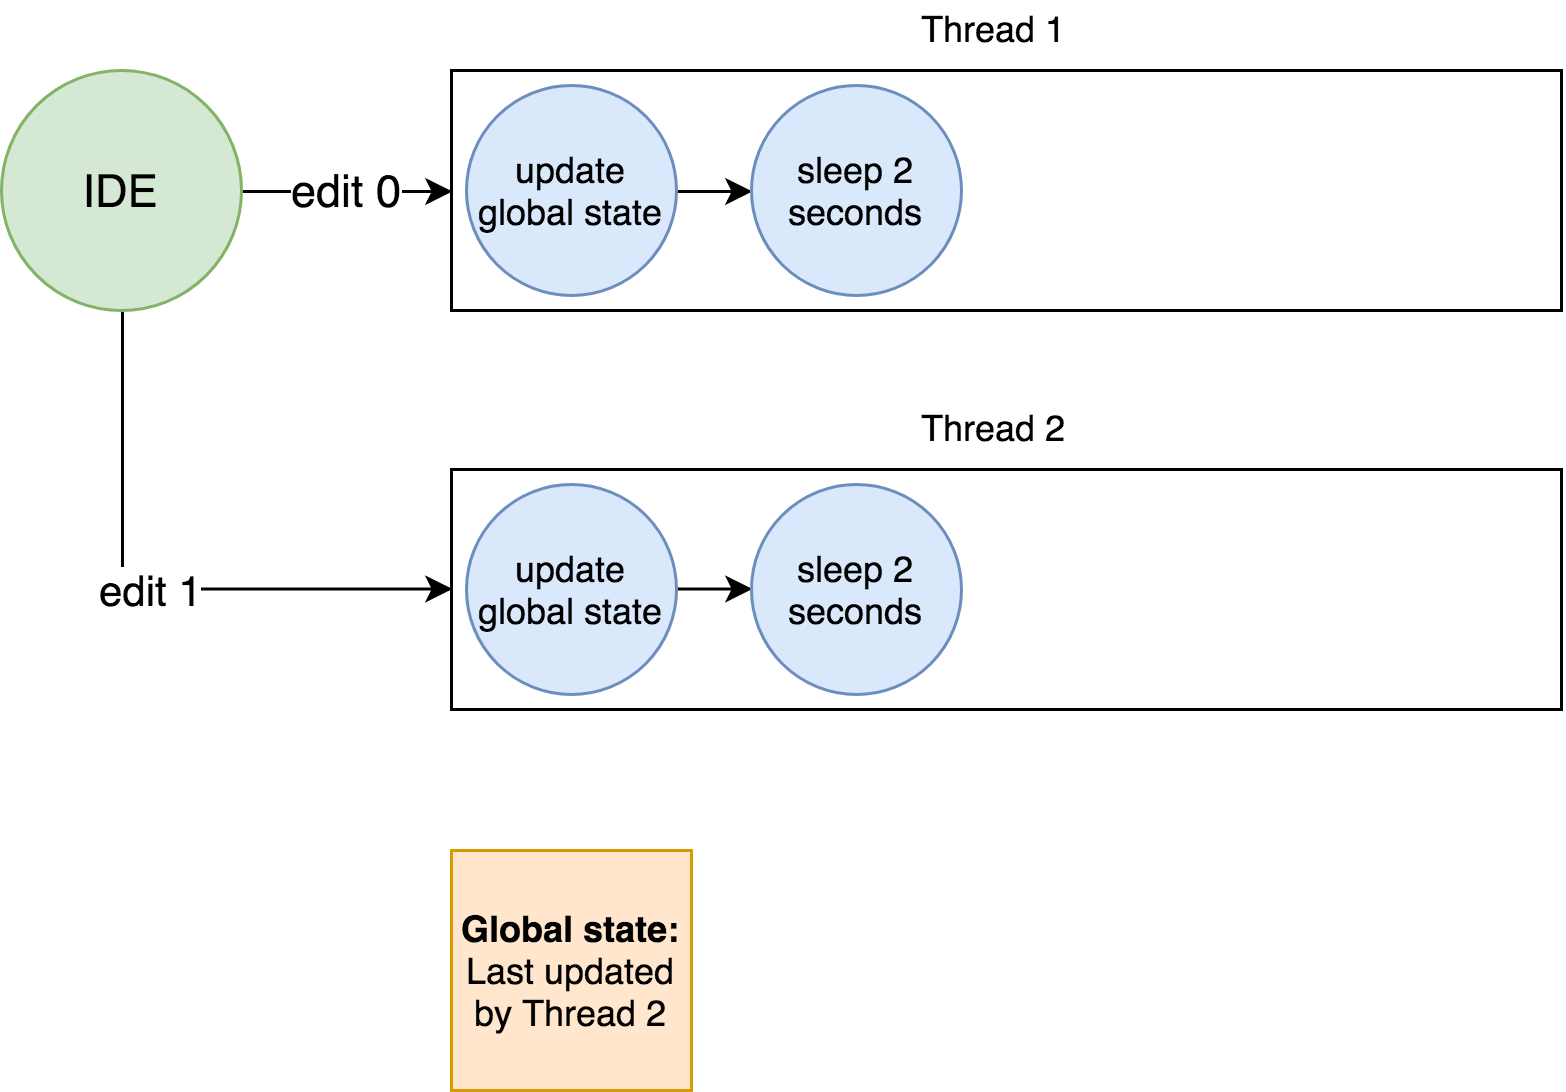
\includegraphics[width=0.6\textwidth]{figures/lsp-step-2.png}
    \caption*{Auto-Compilation Step 2}
\end{figure}
\end{frame}

\begin{frame}
\begin{figure}
\frametitle{LSP - Auto-Compilation}
    \centering
    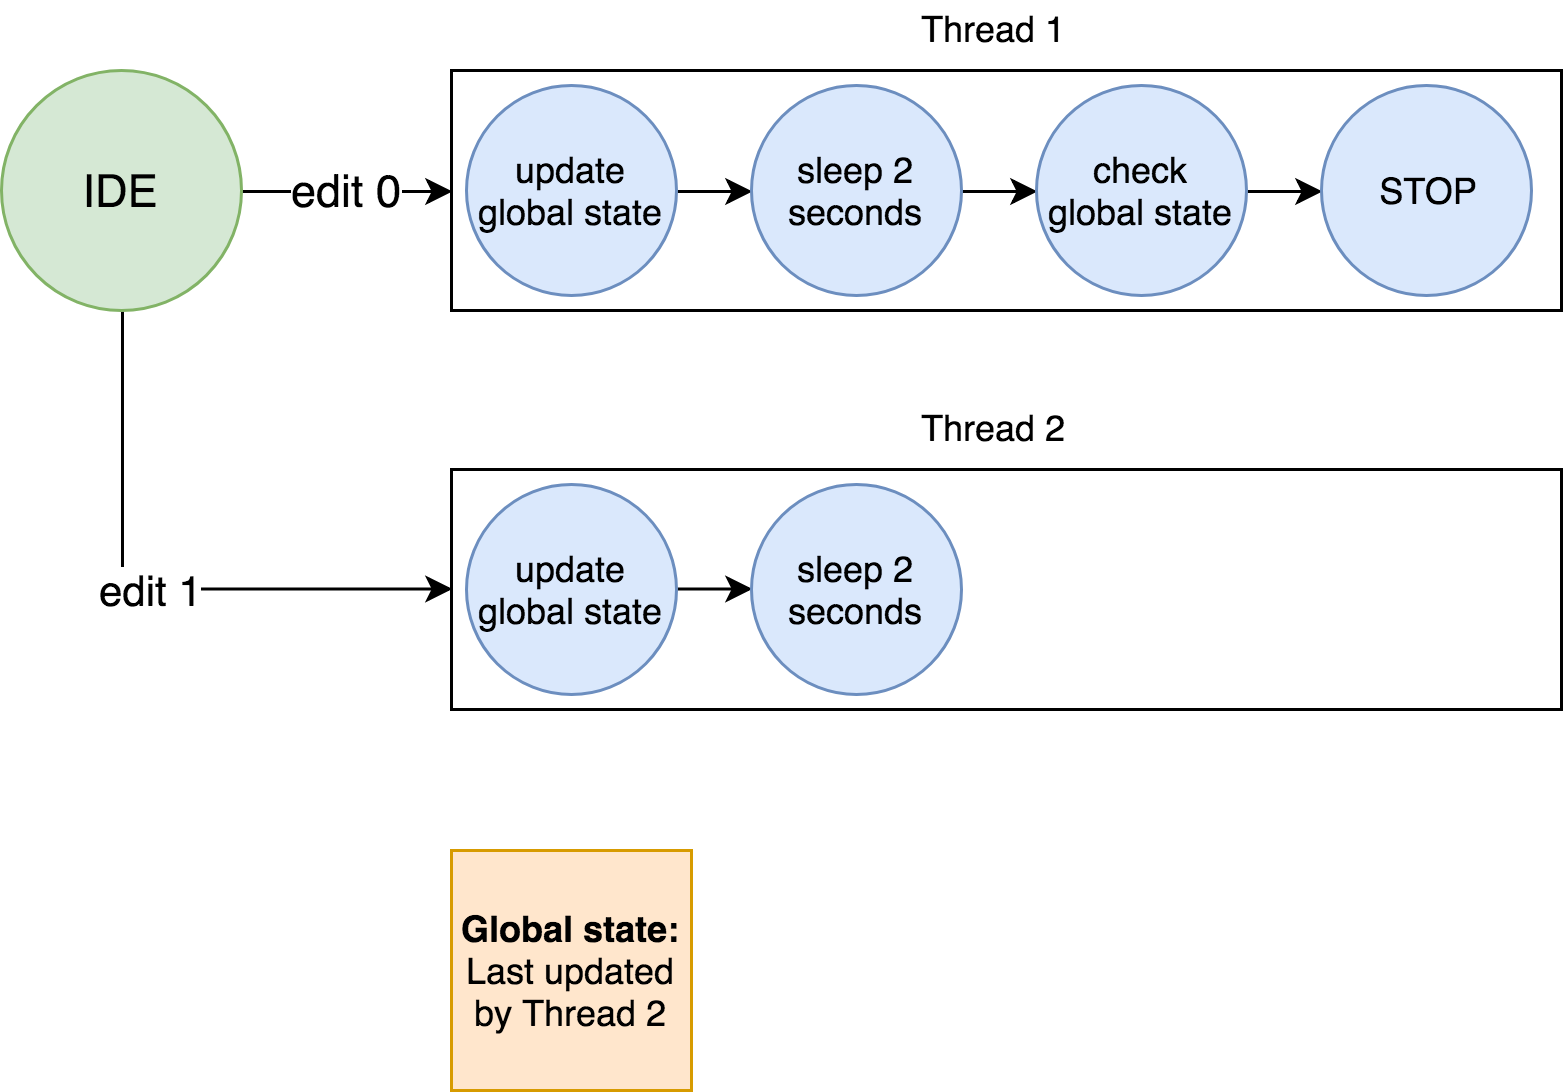
\includegraphics[width=0.6\textwidth]{figures/lsp-step-3.png}
    \caption*{Auto-Compilation Step 3}
\end{figure}
\end{frame}

\begin{frame}
\begin{figure}
\frametitle{LSP - Auto-Compilation}
    \centering
    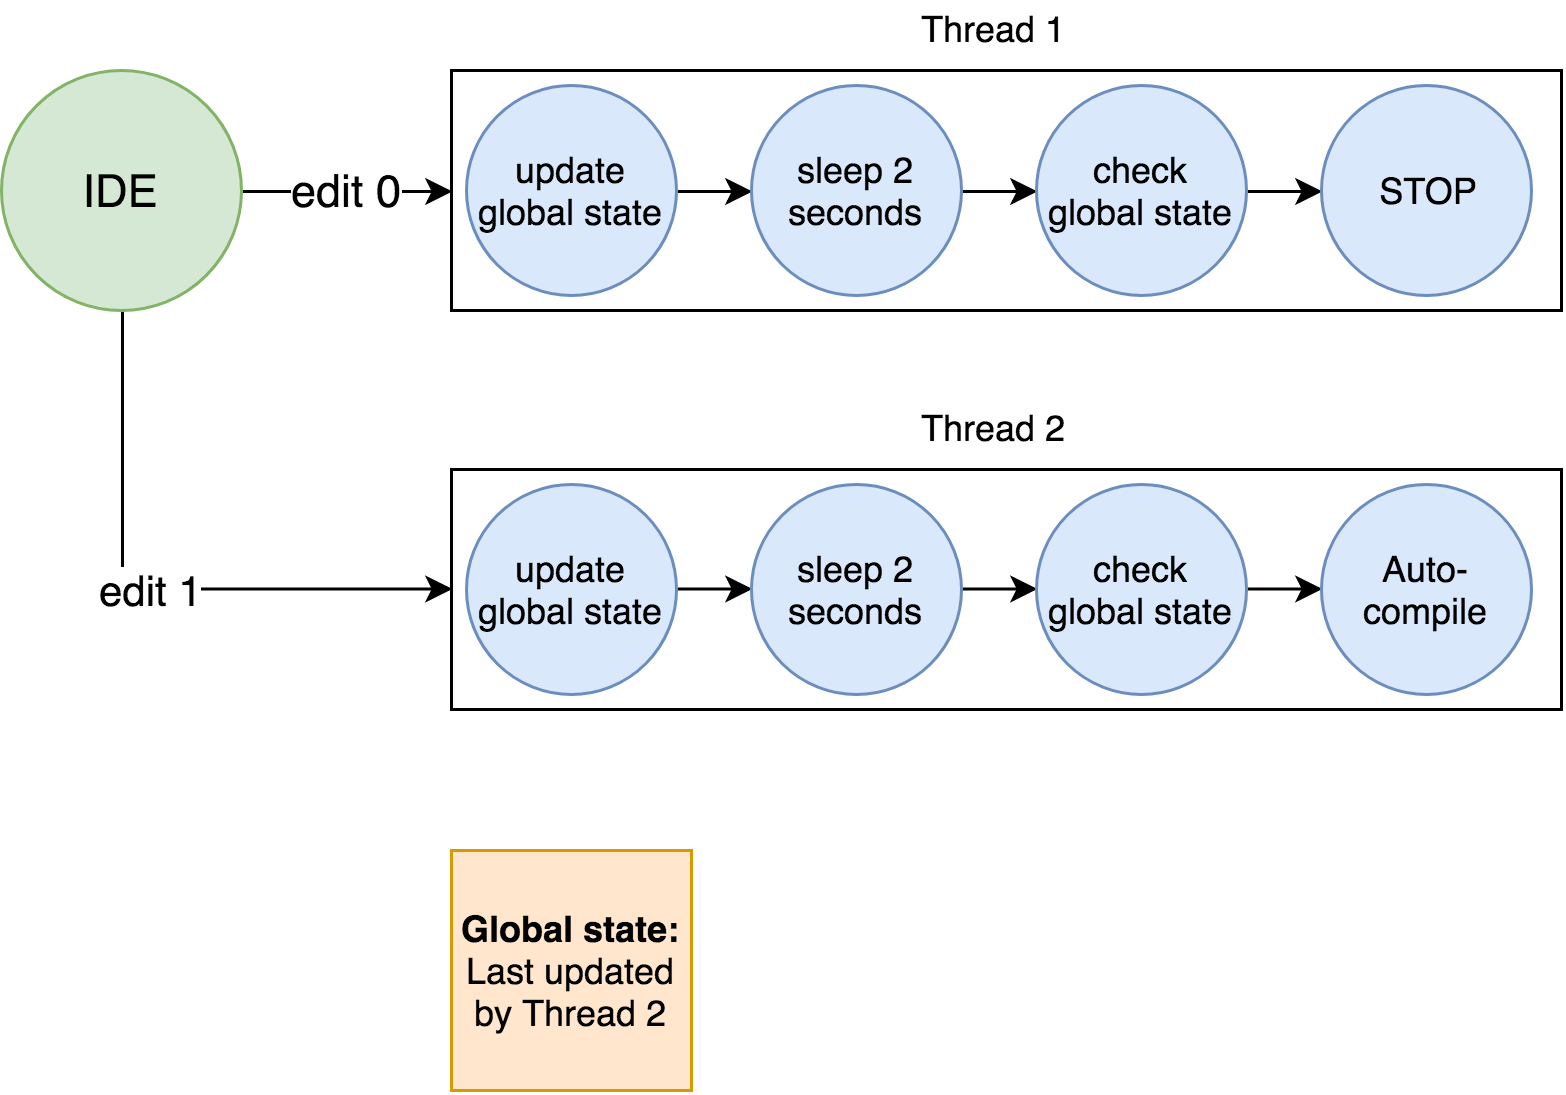
\includegraphics[width=0.6\textwidth]{figures/lsp-step-4.png}
    \caption*{Auto-Compilation Step 4}
\end{figure}
\end{frame}

\subsection{External Calls with Error Handling}

% Ethereum smart contracts are indeed Turing-complete, so it is possible to implement a wide variety of applications in EVM code. Naturally this would not be as useful if smart contracts could only be called by Ethereum users. So in EVM, smart contracts can call other smart contracts. This allows smart contracts to exchange data, but it is at the same time the mechanism used for paying Wei to other contracts.
\begin{frame}{External Calls}
    \begin{itemize}
        \item Smart contracts can represent microservice-like architectures in Ethereum
        \item `Calling' another contract \(\Rightarrow\) data, Gas (computation time), and Wei
    \end{itemize}
\end{frame}

% There are many issues with allowing external calls, however. Ethereum at its core is based around lack of trust. Cryptographic signatures, public ledgers and transactions, verifiable state, etc. all serve to replace trust in other nodes with computation that is hard or impossible to forge. What consequences can an external call have?
% Can a contract be trusted? Not by default, but it may be verified by a third party (do we trust the third party?), or it may be our own.
% Is the interface specified correctly? If not, our external call will go through, but will not call the correct function!
% Will the call fail completely? It may, we need to make sure our own contract handles failures properly.
% What code will the contract run? During an external call, the called contract takes over execution - it can execute any instructions. It does not have access to the state or memory of our (calling) contract, but this is still dangerous, as demonstrated in the following slide (re-entrancy attack).
\begin{frame}{Problems with External Calls}
    \begin{itemize}
        \item Can a contract be trusted?
        \item Is the contract's ABI (interface) specified correctly?
        \item Will the call fail completely?
        \item What code will the contract run?
        \item[$\Rightarrow$] Introducing microservices into a network based on antitrust is dangerous; many Ethereum exploits based around external calls
    \end{itemize}
\end{frame}

% Here is a simple function of a simulated bank. Assume 'balance' contains amounts of Wei owned by some addresses. Now suppose the address 'caller' calls this function to withdraw some money from its attack.
% (for audience, hopefully) What is the problem in this code? Consider the problems highlighted in the previous slide.
\begin{frame}{Re-entrancy Attack}
    \inputminted{swift}{code/reentrancy.flint}
\end{frame}

% This is what the problem is - we can create a contract that exploits this specific bank contract. Recall that transferring money to a contract involves an external call, so the bank has to call 'sendMoney' (or any function) of the 'caller' to give it money. What if 'sendMoney' calls 'bank.withdrawMoney' again? The result is that the bank would run dry of all of its money! Note that the balance of the client is updated AFTER the money is sent - but during this call, the money is requested again and again.
\begin{frame}{Re-entrancy Attack}
    \inputminted{swift}{code/reentrancy2.flint}
\end{frame}

% Unfortunately, we could not solve some problems inherent in Ethereum, not only due to time constraints. However, we aimed to make external calls as safe as possible in Flint.
% Any external contract must have its interface specified using the special external trait syntax. Because the majority of smart contracts on Ethereum are written in Solidity, the Solidity ABI is the network-wide standard for specifying function signatures. This is why types in function signatures use Solidity types (e.g. int256 instead of the Flint Int).
% Any address must be made into an instance of an external trait before it can be used for external calls.
% At the callsite, we specify all the parameters; throughout Flint, parameter labels are required.
% Since we use Solidity types, we introduced casting to convert to and from Flint types. At runtime, these casts make sure that the source value fits into the target type (i.e. 1024 would not successfully cast into int8).
% Notice also the 'value' next to the 'call' keyword - this is how a programmer specifies the amount of Wei to be paid during the external call.
% Finally, every external call must either be in a do-catch block, or be written as 'call!' (hopefully alerting the programmer), which reverts the transaction on failure.
% Compared to Solidity, this is an immense improvement, because Solidity allows type-unsafe calls without interfaces, doesn't force error handling, etc.
\begin{frame}{External Calls in Flint}
    \inputminted{swift}{code/external-calls.flint}
\end{frame}

% (just a summary of the above)
\begin{frame}{External Calls in Flint}
    \begin{itemize}
        \item Type-safe (+ runtime value checks)
        \item Errors revert (\mintinline{swift}{call!}) or have to be handled (\mintinline{swift}{call} in \mintinline{swift}{do ... catch})
        \item `Hyper-parameters' (\texttt{value}, \texttt{gas}) are separate from function arguments
    \end{itemize}
\end{frame}

\subsection{Code Generation}

\begin{frame}{Code Generation}
\centering
Wrong abstraction is the root of all evil.
\end{frame}

\begin{frame}{Nested \texttt{do}-\texttt{catch}}
\begin{columns}
    \begin{column}{0.5\textwidth}
        \inputminted[fontsize=\small]{swift}{code/nested-do.flint}
    \end{column}
    \begin{column}{0.5\textwidth}
        \inputminted[fontsize=\small]{swift}{code/nested-do-catch.flint}
    \end{column}
\end{columns}
\end{frame}

\begin{frame}{Refactor Code Generator}
\begin{itemize}
    \item String concatenation $\Rightarrow$ Representation for YUL IR.
    \item New Emitter API for Codegen adequate for complex code generation.
\end{itemize}
\end{frame}

\sectionslide{Demo}

\sectionslide{Extensions}
% Linear types are a more integrated version of the Asset traits that we have implemented. These types might be implemented with additional syntax and memory operations, allowing variables that hold quantities of an asset that can be split atomically, never duplicated, and never destroyed\cite{flint-paper}. For example, with an asset such as Wei in the context of a @payable contract function, this means we add a semantic check that ensures that the entire value of the incoming asset value is transferred to another instance to prevent its destruction.
\subsection{Linear Types}

\begin{frame}
\frametitle{Linear Types}
\begin{itemize}
    \item Treating assets as integer values is a source of numerous bugs and exploits not only on the Ethereum network
    \item Linear types would be integrated into the language to never allow an asset to be destroyed, duplicated, or created from scratch
\end{itemize}
\end{frame}

\begin{frame}
\frametitle{Linear Types Example}
\inputminted{swift}{code/linear-types.flint}
\end{frame}


\subsection{Modularisation}
% Adding modules allows a contract definition to be split across multiple source files and for the inclusion and distribution of user-made libraries and frameworks.

\begin{frame}
\frametitle{Modularisation}
Allows more complex contracts to be split into multiple files \\
\inputminted{swift}{code/modularisation.flint}
\end{frame}

% A package manager has long been a requested feature, but until we implemented external calls there was no reason to have one because there would've been no way to call another contract. Additionally, since the language does not currently support modules, there is no way to import code from another Flint program. Once modules and a Flint ABI are supported, there will be a better case for having a package manager.
\subsection{Package Manager}

\begin{frame}
\frametitle{Package Manager}
\begin{itemize}
    \item A smart contract tracking deployed Flint contracts
    \item Would allow modules to be imported from addresses in a type-safe manner
\end{itemize}
\end{frame}

\begin{frame}
\frametitle{Package Manager Example}
\inputminted{swift}{code/fpm.flint}
\end{frame}

\sectionslide{Conclusion}
%
% We would like to conclude by summarising our work and what we have learnt.
% By adding external calls and exception handling to the language we have made
% Flint much more usable and able to interact with the real world.
% By adding - amongst other features - Asset traits, we have added a feature that
% will make Flint more useful than languages like Solidity in the future.
% The Language Server Protocol implementation has hugely improved the Flint ecosystem.
% In doing all this, we have learnt a lot; not just about the Ethereum-specific parts
% but of course about compiler development and more generally about software engineering.
% Still, there is a lot more interesting work to be done to make smart contracts safer.
%
\begin{frame}{Conclusion}
    \begin{center}
        \begin{itemize}
            \item We added features that make Flint more \textbf{usable}
            \item We added features that make Flint more \textbf{useful}
            \item We learned a lot about the \textbf{Ethereum ecosystem}, \textbf{compiler development} and \textbf{software engineering}
            \item There is huge potential for \textbf{further improvements}, in particular as the Ethereum ecosystem evolves
        \end{itemize}
    \end{center}
\end{frame}

\begin{frame}
 	\vbox{}
	\begin{center}
	\LARGE\usebeamercolor[fg]{title} Thank you for your attention
	\end{center}
\end{frame}
%﷽﷽ FIN ﷽﷽
%﷽﷽ FIN ﷽﷽
%﷽﷽ FIN ﷽﷽
%﷽﷽ FIN ﷽﷽

\end{document}